\section{Introduction to Statics}

\subsection{Newton's Laws}

\blue{From TAM212 Reference Pages (Kinetics of Point Masses - Newton's Equations):}


Newton's equations relate the acceleration $\vec{a}$ of a point mass with mass $m$ to the total applied force $\vec{F}$ on the mass (sum of all applied forces). There is no derivation for Newton's equations, because they are an assumed model for dynamics. We can only verify them by comparing with experimental evidence, which confirms that Newtonian dynamics are accurate for non-relativistic and non-quantum systems.

They are:

\subsubsection{Newton's First Law}

A particle at rest stays that way unless acted on by unbalanced forces. 

\subsubsection{Newton's Second Law}

\[\vec{F} = m \vec{a}\]

\subsubsection{Newton's Third Law}

The mutual forces of action and reaction between two particles are equal, opposite, and collinear. 

\subsubsection{Example}

\begin{figure*}[!h]
\centering
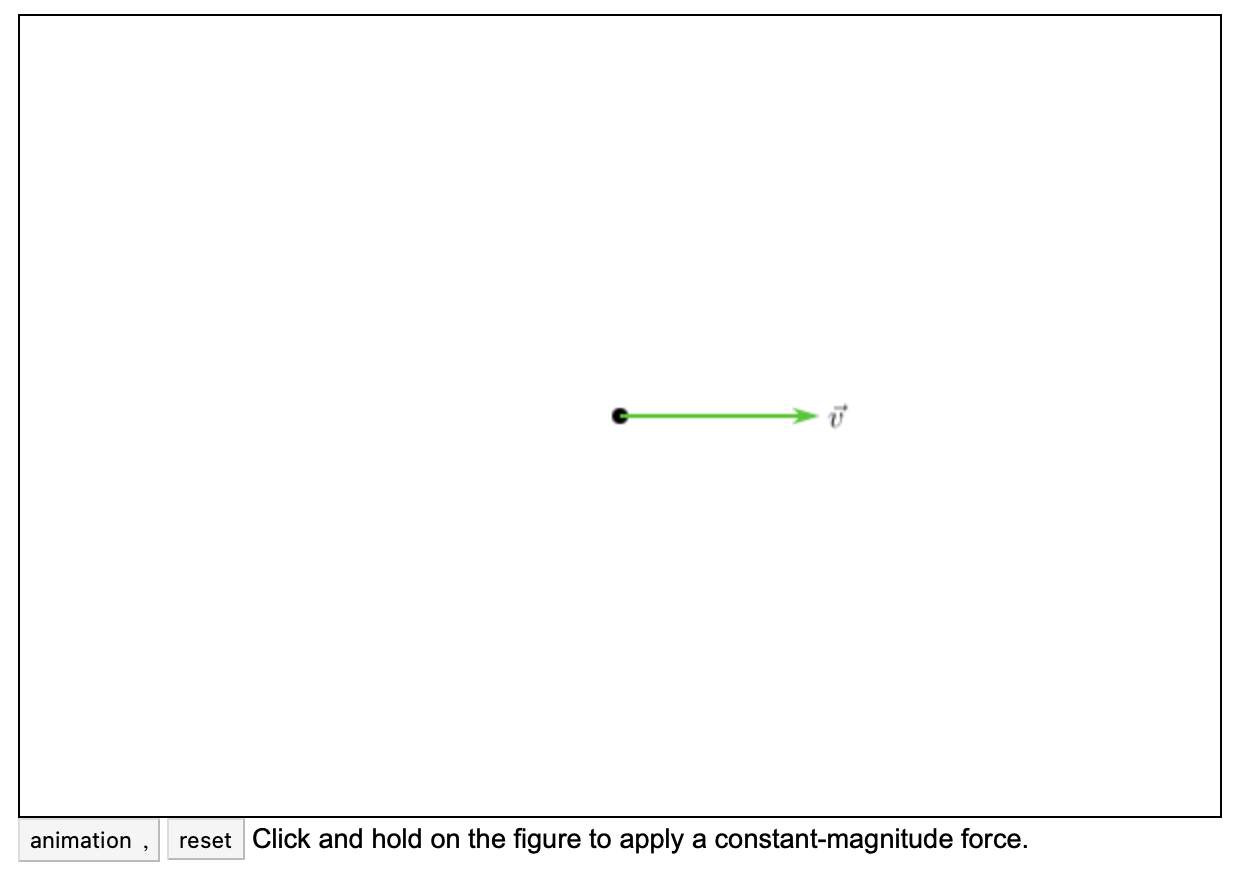
\includegraphics[angle=0, width=5in]{IntroductionFigures/NewtonsLaws.png}
\vspace{-2mm}
\caption{\small \blue{Taken from TAM212 Reference Pages (Kinetics of Point Masses - Newton's Equations)}}
\vspace{-3mm}
\label{Fig:NewtonsLaws}
\end{figure*}

\subsection{Idealizations}

\subsubsection{Particles}
%Could change this section to "Idealizations" and write about particle idealizations, rigid body assumptions, and concentrated / distributed force assumptions. 

In this course, we assume two things about particles: 

\begin{enumerate}
    \item{The mass of the particle is not 0.}
    \item{The radius of the mass is 0.}
\end{enumerate}

\noindent Through these assumptions, we are essentially concentrating all of the mass of an object at a single point in space. The particle has a mass but the size and shape of the particle is not taken into account. 

\subsubsection{Rigid Bodies}

For rigid bodies, we assume that the object has both mass (similar to particles) but also take its shape into account. 

We call these bodies "rigid" because we assume that they do not deform under applied forces or moments. 

\blue{Insert the same content here as from the TAM212 Reference Pages (Rigid Bodies - introductory section at the top of the page).}

